\section{The role of the solar apex}

% References: http://burro.cwru.edu/Academics/Astr222/Galaxy/Kinematics/solarmotion.html

Interstellar objects can be discovered from various directions in space.
However, it is more common for them to be detected near the direction of the
solar apex, as observed with 1I/'Oumuamua (in the constellation Lyra) and 2I/Borisov
(in the constellation Cassiopeia).

The solar apex, also known as the apex of the Sun's motion, indicates the
direction in which the Sun is traveling relative to the local standard of rest
(LSR). Positioned in the constellation Hercules, southwest of the bright star
Vega, its visual coordinates are right ascension 18h 28m 0s and declination +30°
N. The solar apex moves at a velocity of approximately 19.4 km/s (4.09 AU/year)
relative to the local standard of rest, see \cite{dehnen1998}. Conversely, the
solar antapex, situated near the star Zeta Canis Majoris in the constellation
Columba, points in the opposite direction. Due to this high relative speed,
encounters with intersellar objects are more likely to occur in the direction of
the solar apex and present hyperbolic orbits.

Figure \ref{fig:solar_apex} illustrates the locations of the solar apex and
antapex. The radial velocities of nearby stars are denoted by $V_r$, while their
proper motions are represented by $\mu$.

\begin{figure}[H]
  \centering
  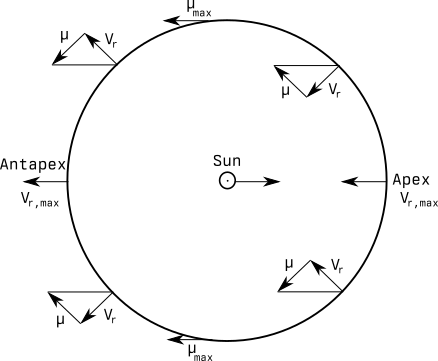
\includegraphics[width=0.5\textwidth]{static/solar_apex.png}
  \caption[The motion of the Sun in the LST.]
  {
    The motion of the Sun in the LST. The apex and antiapex are
    represented in the same and opposite direction of the Sun's motion.
    The combination of radial veolcities and proper motions of stars in the
    leads to the apparent motion of stars in the LST moving from the apex
    towards the antiapex.
  }
  \label{fig:solar_apex}
\end{figure}

As the Sun progresses towards the solar apex, nearby stars appear to diverge
from this point in the celestial sphere. Conversely, stars seem to converge
towards each other in the direction of the solar antapex.

It is important to note that the Sun's motion within the Milky Way galaxy is not
solely restricted to the galactic plane; it also entails an oscillatory movement
relative to the plane spanning millions of years.

Authors like \cite{marceta2023} consider the role of the solar apex when
generating a synthetic population of interstellar objects in the solar system.
Figure \ref{fig:distribution_interlopers} shows the expected distribution of
interlopers.

\vspace{1cm}

\begin{figure}[H]
  \centering
  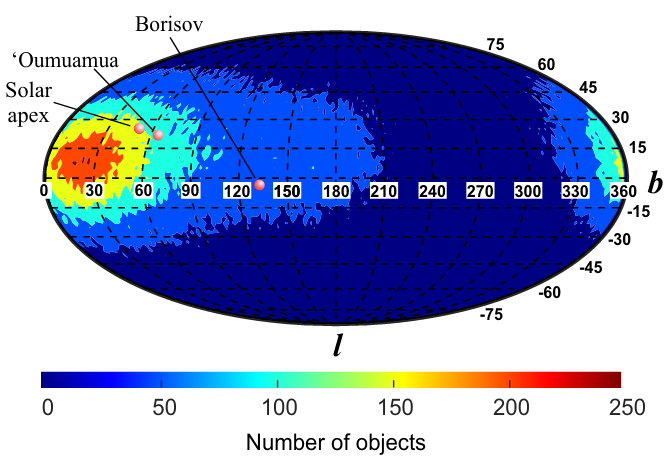
\includegraphics[width=0.9\textwidth]{static/distribution_interlopers.png}
  \caption[Expected interlopers distribution in the solar system.]{The
    expected distribution of interlopers in the solar system, represented in
    a galactic coordinates. A higher density of interlopers is expected in
    the direction of the solar apex. The direction of 1I/'Oumuamua and 2I/Borisov
    is found to be close to this point, located near constellation Lyra.
    This contour plot is figure 11 of \cite{marceta2023} article. It is
    reproduced under permission of its original author.
  }
  \label{fig:distribution_interlopers}
\end{figure}

Despite this preferred direction, it is important to remember that there is
nothing that prevents and ISO to be discovered in other direction. In fact,
probabilities for intetifying an interloper approaching in the direction of the
solar-antapex are lower, but not null.
